\chapter{扩展:改进Poisson求解器}
\label{ch:poisson}


\begin{quote}
我们迄今为止撰写的FENICS计划已经设计为平面设计
Python脚本。 这对于解决简单的演示非常有用
问题。 但是,当您构建高级的求解器时
应用程序,你会很快找到需要更多的结构化
节目。 特别是,您可能希望重用您的求解器来解决
大量的问题,你们改变边界条件,
域,以及材料参数等系数。 在本章中,
我们将看到如何编写一般的求解器函数来改进
FEniCS计划的可用性。 我们也会讨论如何
利用具有预处理器的迭代求解器来求解线性
系统,如何计算派生数量,例如通量
在边界的一部分,以及如何计算错误和收敛
率。
\end{quote}

\section{重构Poisson求解器}
\label{ch:poisson0:impl2}

\index{flat program}

本书中讨论的大多数程序是“平”就是他们是
在Python方面没有组织成逻辑,可重复使用的单位
功能。这样的平面程序对于快速测试想法是有用的
素描解算法,但不适合严重
解决问题因此,我们将看看如何\emph{refactor}
Poisson求解器从Chapter~\ref{ch:fundamentals}。一开始就这样
意味着将代码分解为函数。但重构不仅仅是一个
重新排列现有声明。在重构期间,我们也尝试
使我们创建的功能尽可能在其他方面可重用
上下文。我们也会封装一些具体的陈述
问题变成(不可重用)的功能。能够区分
当重构时,专用代码的可重用代码是一个关键问题
代码,这个能力取决于一个很好的数学理解
手头的问题(什么是一般的,什么是特殊的)。在一个单位
程序,一般和专门的代码(和数学)经常
混合在一起,这往往会给人一种模糊的理解
手头的问题。

\subsection{更一般的求解器函数}
\label{ch:poisson0:impl2:func}

我们考虑平面计划
\begin{center}
\url{https://fenicsproject.org/pub/tutorial/python/vol1/ft01_poisson.py}
\end{center}
解决了Poisson问题的开发
在章节~\ref{ch:fundamentals}。
这个程序中的一些代码
需要解决任何Poisson问题$-\nabla^2 u=f$ on $[0,1]\times
[0,1]$与$u=\ub$在边界上,而其他语句来自
我们简单的测试问题。 让我们收集一般的,可重复使用的代码
一个名为\texttt{solver}的函数。 我们的特殊测试问题就是这样
我们的\texttt{solver}的一个应用程序附加了一些其他语句。 我们限制
\texttt{solver}函数来计算数值
解。 绘制和比较解决方案与确切的解决方案
被认为是要执行的特定于问题的活动
别处。

我们将\texttt{solver}参数化为$f$, $\ub$和分辨率
目。 因为使用高阶有限元是如此微不足道
函数通过将第三个参数改为\texttt{FunctionSpace},我们
还加入有限元函数空间的多项式度
作为\texttt{solver}的参数。

\begin{python}
from fenics import *
import numpy as np

def solver(f, u_D, Nx, Ny, degree=1):
    """
    Solve -Laplace(u) = f on [0,1] x [0,1] with 2*Nx*Ny Lagrange
    elements of specified degree and u = u_D (Expresssion) on
    the boundary.
    """

    # Create mesh and define function space
    mesh = UnitSquareMesh(Nx, Ny)
    V = FunctionSpace(mesh, 'P', degree)

    # Define boundary condition
    def boundary(x, on_boundary):
        return on_boundary

    bc = DirichletBC(V, u_D, boundary)

    # Define variational problem
    u = TrialFunction(V)
    v = TestFunction(V)
    a = dot(grad(u), grad(v))*dx
    L = f*v*dx

    # Compute solution
    u = Function(V)
    solve(a == L, u, bc)

    return u
\end{python}

我们的初始程序的其余任务,如调用\texttt{solver}
功能与问题特定的参数和绘图,
可以放在一个单独的功能。 这里我们选择放这个代码
在一个名为\verb!run_solver!的函数中:

\begin{python}
def run_solver():
    "Run solver to compute and post-process solution"

    # Set up problem parameters and call solver
    u_D = Expression('1 + x[0]*x[0] + 2*x[1]*x[1]', degree=2)
    f = Constant(-6.0)
    u = solver(f, u_D, 8, 8, 1)

    # Plot solution and mesh
    plot(u)
    plot(u.function_space().mesh())

    # Save solution to file in VTK format
    vtkfile = File('poisson_solver/solution.pvd')
    vtkfile << u
\end{python}

该解决方案现在可以被计算,绘制和保存到文件
只需调用\verb!run_solver! 功能。

\subsection{将求解器写为Python模块}

\index{Python module}

重构的代码放在一个文件中
\begin{center}
\url{https://fenicsproject.org/pub/tutorial/python/vol1/ft12_poisson_solver.py}。
\end{center}
我们应该确保这样的文件可以导入(因此
重用)在其他程序。 这意味着所有的语句在主
不在功能内的程序应该出现在测试中
\verb!if __name__ == '__main__':! 如果文件被执行,则该测试是真实的
一个程序,但是假的如果导入文件。 如果我们想运行这个
文件的方式与我们可以运行\verb!ft01_poisson.py!,相同
主程序只是一个调用\verb!run_solver! 其次是电话
\texttt{interactive}保存情节:

\begin{python}
if __name__ == '__main__':
    run_solver()
    interactive()
\end{python}
这个完整的程序可以在文件中找到
\begin{center}
\url{https://fenicsproject.org/pub/tutorial/python/vol1/ft12_poisson_solver.py}。
\end{center}

\index{ft12\_poisson\_solver.py@{\rm\texttt{ft12\_poisson\_solver.py}}}
\index{unit testing}

\subsection{验证和单元测试}

\index{verification}

我们的第一个程序的剩余部分是比较数字
和确切的解决方案。 每次我们编辑代码,我们必须重新运行
测试并检查\verb!error_max! 足够小,所以我们知道
该代码仍然有效。 为此,我们将采用单元测试,
意味着我们创建了一个数学测试和相应的软件
可以自动运行所有测试,并检查所有测试
通过。 Python有几个单元测试工具。 两个很受欢迎
一个是pytest和nose。 这几乎是一样的,非常容易
使用。 通过测试类提供更经典的单元测试
内置模块\texttt{unittest},但是这里我们要使用pytest
(或nose),因为这将导致更短和更清晰的代码。

在数学上,我们的单元测试是有限元解
我们的问题当$f=-6$等于确切的解决方案$u=\ub=1+x^2+2y^2$
在网格的顶点。
我们已经创建了一个在顶点找到错误的代码
我们的数值解。 由于四舍五入的错误,我们不能要求这个
错误为零,但是我们必须使用一个容差,哪个
取决于元素的数量和多项式的程度
在有限元的基础上。 如果我们要测试那个
\texttt{solver}函数适用于高达$2\times(20\times 20)$的网格
元素和立方体Lagrange元素,$10^{-10}$是适当的
容忍测试最大误差消失。

为了使我们的测试用例与pytest和nose一起工作,我们必须
对我们的程序进行几个小的调整。 简单
规则是每个测试都必须放在一个函数中

\begin{itemize}
 \item 名字以\verb!test_!开头

 \item 没有论据,

 \item 执行表示为\texttt{assert success, msg}的测试。
\end{itemize}

\noindent
关于最后一点,\texttt{success}是一个布尔表达式
\texttt{False}如果测试失败,在这种情况下,字符串\texttt{msg}是
写入屏幕。 当测试失败时,\texttt{assert}会引发一个
Python中的\texttt{AssertionError}异常,否则运行
默默。 \texttt{msg}字符串是可选的,所以\texttt{assert success}是
最小测试。 在我们的例子中,我们会写\verb!assert error_max <tol!,
其中\texttt{tol}是上述容限。

在该单元测试中执行适当的测试功能
pytest或nose测试框架具有以下形式。 注意
我们对不同的网格分辨率和度数执行测试
有限元。

\begin{python}
def test_solver():
    "Test solver by reproducing u = 1 + x^2 + 2y^2"

    # Set up parameters for testing
    tol = 1E-10
    u_D = Expression('1 + x[0]*x[0] + 2*x[1]*x[1]', degree=2)
    f = Constant(-6.0)

    # Iterate over mesh sizes and degrees
    for Nx, Ny in [(3, 3), (3, 5), (5, 3), (20, 20)]:
        for degree in 1, 2, 3:
            print('Solving on a 2 x (%d x %d) mesh with P%d elements.'
                  % (Nx, Ny, degree))

            # Compute solution
            u = solver(f, u_D, Nx, Ny, degree)

            # Extract the mesh
            mesh = u.function_space().mesh()

            # Compute maximum error at vertices
            vertex_values_u_D = u_D.compute_vertex_values(mesh)
            vertex_values_u  = u.compute_vertex_values(mesh)
            error_max = np.max(np.abs(vertex_values_u_D - \
                                      vertex_values_u))

            # Check maximum error
            msg = 'error_max = %g' % error_max
            assert error_max < tol, msg
\end{python}

要运行测试,我们键入以下命令:

\begin{bash}
$ py.test ft12_poisson_solver.py
\end{bash}
这将运行所有名为\verb!test_ *!的函数(目前只有
\verb!test_solver!函数)在文件中找到并报告结果。
对于更详细的输出,请添加flags \texttt{-s -v}。

我们将会习惯于将数字测试问题包含进来
单元测试如上,我们强烈鼓励读者创建
每当实施FEniCS求解器时,进行类似的单元测试。

\begin{notice}[提示:在测试功能中打印消息]
当测试通过时,\texttt{assert}语句静默运行,以便用户可以
测试功能中的所有语句是否真的会变得不确定
执行。 心理帮助是在\texttt{assert}之前打印出一些东西
(正如我们在上面的例子中所做的那样),这样很清楚
测试真的发生了。
请注意,\texttt{py.test}需要\texttt{-s}选项来显示打印输出
从测试功能。
\end{notice}

\begin{notice}[提示:使用iPython进行调试]
可以通过添加以下内容从Python脚本轻松输入iPython
代码中的任何位置:
\begin{python}
from IPython import embed; embed()
\end{python}
这一行开始一个交互式的Python会话,让你
打印和绘图变量,这对调试非常有帮助。
\end{notice}

\subsection{参数化空间维数}
\label{ch:poisson0:nD}
\index{dimension-independent code}

\index{space dimensions}

FEniCS可以很容易地编写一个可以统一的模拟代码
操作在1D,2D和3D。 作为开胃菜,回到
以前的节目
\begin{center}
\url{https://fenicsproject.org/pub/tutorial/python/vol1/ft01_poisson.py}
要么
\url{https://fenicsproject.org/pub/tutorial/python/vol1/ft12_poisson_solver.py}
\end{center}
并将网格构造从\texttt{UnitSquareMesh(8,8)}更改为
\texttt{UnitCubeMesh(8,8,8)}。 现在域是单位立方体
分为$8\times 8\times 8$
盒子和每个盒子
分为六个四面体形有限元
计算。 运行程序,观察我们可以解决3D
问题没有任何其他修改! (在1D中,表达式必须是
修改为不依赖于\texttt{x [1]})。可视化允许你
旋转立方体并观察功能值作为颜色
边界。

如果我们要参数化单位间隔的创建,单位平方,
或单位立方体尺寸,我们可以通过封装这部分来实现
的函数中的代码。 给定一个列表或元组指定除法
进入空格坐标中的单元格,具有以下功能
返回$d$维数多维数据集的网格:

\begin{python}
def UnitHyperCube(divisions):
    mesh_classes = [UnitIntervalMesh, UnitSquareMesh, UnitCubeMesh]
    d = len(divisions)
    mesh = mesh_classes[d - 1](*divisions)
    return mesh
\end{python}
施工\verb!mesh_class[d - 1]! 会选出正确的名字
用于定义域并生成网格的对象。 而且,
参数\texttt{* divisions}发送列表的所有组件\texttt{divisions}
作为网格构造的构造函数的单独参数
类由\verb!mesh_class[d - 1]!挑选出来。 例如,在2D问题中
其中\texttt{divisions}有两个元素,即语句

\begin{python}
mesh = mesh_classes[d - 1](*divisions)
\end{python}
相当于

\begin{python}
mesh = UnitSquareMesh(divisions[0], divisions[1])
\end{python}

\texttt{solver}函数
\begin{center}
\url{https://fenicsproject.org/pub/tutorial/python/vol1/ft12_poisson_solver.py}
\end{center}
可以通过替换来修改$d$维度问题
\texttt{Nx}和\texttt{Ny}参数由\texttt{divisions}调用,并调用该函数
\texttt{UnitHyperCube}创建网格。 注意\texttt{UnitHyperCube}是一个
\emph{function}而不是\emph{class},但是我们使用所谓的命名它
\emph{CamelCase符号}使其看起来像一个类:

\begin{python}
mesh = UnitHyperCube(divisions)
\end{python}

\section{使用线性求解器}
\label{ch:poisson0:solve:prm}

默认使用稀疏LU分解(Gaussian消除)
在FEniCS程序中求解线性方程组。 这是非常
鲁棒简单的方法。 这是系统的推荐方法
最多有几千个未知数,因此可能是其中的一种
许多2D和更小的3D问题的选择。 但是,稀疏LU
分解变慢,一个快速耗尽内存
更大的问题 对于大问题,我们需要使用\emph{iterative
方法}它们更快,需要更少的内存。 我们现在
看看如何利用最先进的迭代解决方案
FEniCS中的方法。

\subsection{选择线性求解器和预处理器}

\index{linear solver}
\index{preconditioner}
\index{Krylov solver}

预处理Krylov求解器是一种流行的迭代方法
在FEniCS程序中可以轻松访问。 Poisson方程
产生一个对称的正定系统矩阵,为此,
最优Krylov求解器是Conjugate Gradient(CG)方法。 对于
非对称问题,非对称系统的Krylov求解器,
如GMRES,是一个更好的选择。 不完整LU分解(ILU)
是一个流行和强大的全面预处理器,所以让我们试试
GMRES-ILU对:

\begin{python}
solve(a == L, u, bc,
      solver_parameters={'linear_solver': 'gmres',
                         'preconditioner': 'ilu'})
# Alternative syntax
solve(a == L, u, bc,
      solver_parameters=dict(linear_solver='gmres',
                             preconditioner='ilu'))
\end{python}
部分~\ref{ftut:app:solver:prec}列出了最受欢迎的选择
Krylov解决方案和预处理器可用于FEniCS。

\index{linear algebra backend}
\index{PETSc} \index{Eigen}

\subsection{选择线性代数后端}

实际的GMRES和ILU实施被采取行动
取决于线性代数包的选择。 FEniCS接口
几个线性代数包,称为\emph{linear algebra backends}
FEniCS术语。 如果FEniCS被编译,PETSc是默认选择
与PETSc。 如果PETSc不可用,则FEniCS将回退使用
Eigen后端。 FEniCS中的线性代数后端可以设置
使用以下命令:

\begin{python}
parameters.linear_algebra_backend = backendname
\end{python}
\texttt{backendname}是一个字符串。 查看哪个线性代数后端
可用,您可以调用FEniCS功能\\
\verb!list_linear_algebra_backends! 同样,可以查看哪一个
线性代数后端正在被以下使用
命令:

\begin{python}
print(parameters.linear_algebra_backend)
\end{python}

\index{parameters@{\rm\texttt{parameters}}}
\index{info@{\rm\texttt{info}}}

\subsection{设置求解器参数}

我们通常会在停止时控制容差
标准和运行时的最大迭代次数
迭代法 这样的参数可以在全局控制
和地方一级。 我们将从如何设定全球化开始
参数。 对于更高级的程序,可能需要使用一个数字
的不同线性求解器并设置不同的公差等
参数。 那么在a处控制参数变得很重要
地方一级。 我们将在~\ref{ch:poisson0:solver:problem}部分中回到此问题。

更改全局FEniCS参数数据库中的参数会影响
所有线性求解器(在参数设置后创建)。
全局FEniCS参数数据库简称为\texttt{parameters}和
它表现为一个嵌套字典。 写

\begin{python}
info(parameters, verbose=True)
\end{python}
列出数据库中的所有参数及其默认值。
参数集的嵌套通过缩进表示
从\texttt{info}输出。
根据该输出,相关参数集为
命名为\verb!'krylov_solver'!,参数设置如下:

\begin{python}
prm = parameters.krylov_solver  # short form
prm.absolute_tolerance = 1E-10
prm.relative_tolerance = 1E-6
prm.maximum_iterations = 1000
\end{python}
针对Krylov求解器的停止标准通常涉及一些规范
剩余值必须小于绝对公差
参数或小于相对公差参数次数
初始残留。

我们注意到,全局参数数据库的默认值可以是
在XML文件中定义。 从当前集合生成这样的文件
的程序中的参数,运行

\begin{python}
File('parameters.xml') << parameters
\end{python}
如果一个\verb!dolfin_parameters.xml! 文件在目录中找到
运行FEniCS程序,该文件被读取并用于初始化
\texttt{parameters}对象。 否则,该文件
\verb!.config/fenics/dolfin_parameters.xml!
在用户的主目录是
阅读,如果存在。 另一个选择是加载XML文件(与任何
名称)手动在程序中:

\begin{python}
File('parameters.xml') >> parameters
\end{python}
XML文件也可以是gzip的形式,扩展名为\texttt{.xml.gz}。

\subsection{扩展求解器函数}

我们可能会扩展以前的求解器函数
\begin{center}
\url{https://fenicsproject.org/pub/tutorial/python/vol1/ft12_poisson_solver.py}
\end{center}
在部分〜\ref{ch:poisson0:impl2:func}
这样它也提供了GMRES + ILU
预处理Krylov求解器:

\index{ft10\_poisson\_extended.py@{\rm\texttt{ft10\_poisson\_extended.py}}}

这个新的\texttt{solver}函数在文件中找到
\begin{center}
\url{https://fenicsproject.org/pub/tutorial/python/vol1/ft10_poisson_extended.py},
取而代之
\url{https://fenicsproject.org/pub/tutorial/python/vol1/ft12_poisson_solver.py}。
\end{center}
它具有以前\texttt{solver}功能的所有功能,但是
也可以用迭代法解决线性系统。

subsection{关于单元测试的评论}

关于以单位来验证新的\texttt{solver}函数
测试,事实证明单位测试的问题在哪里
当我们使用时,近似误差消失会变得更加复杂
迭代方法。问题是由于迭代而保持错误
解决方案小于验证中使用的公差
试验。首先,这意味着Krylov中使用的公差
求解器必须小于\texttt{assert}测试中使用的公差,
但是这并不能保证线性求解误差小。
对于线性元素和小网格,容差为$10^{-11}$作品
在Krylov求解器的情况下(使用容限$10^{-12}$)
在那些解答者)。有兴趣的读者参考
\verb!demo_solvers!功能在
\begin{center}
\url{https://fenicsproject.org/pub/tutorial/python/vol1/ft10_poisson_extended.py}
\end{center}
详情请见:
该函数测试直接和迭代的数值解
线性求解器,适用于不同网格,不同程度的
有限元基函数中的多项式。

\subsection{线性求解器方法和预处理器列表}
\label{ftut:app:solver:prec}

\index{linear solver}
\index{Krylov solver}
\index{preconditioner}

哪些线性求解器和预处理器可用
在FEniCS中取决于FEniCS的配置以及哪些
线性代数后端当前处于活动状态。 下表
显示了可用的线性求解器的示例
当PETSc后端处于活动状态时,通过FEniCS:

{\small

\vspace{4mm}

\begin{tabular}{ll}
\hline\noalign{\smallskip}
\multicolumn{1}{c}{ 名称 } & \multicolumn{1}{c}{ 方法 } \\
\noalign{\smallskip}\hline\noalign{\smallskip}
\texttt{'bicgstab'}     & Biconjugate gradient stabilized method       \\
\texttt{'cg'}           & Conjugate gradient method                    \\
\texttt{'gmres'}        & Generalized minimal residual method          \\
\texttt{'minres'}       & Minimal residual method                      \\
\texttt{'petsc'}        & PETSc built in LU solver                     \\
\texttt{'richardson'}   & Richardson method                            \\
\verb!'superlu_dist'! & Parallel SuperLU                             \\
\texttt{'tfqmr'}        & Transpose-free quasi-minimal residual method \\
\texttt{'umfpack'}      & UMFPACK                                      \\
\noalign{\smallskip}\hline\noalign{\smallskip}
\end{tabular}

\vspace{4mm}

}

\noindent
该组可用的预处理器还取决于配置和
线性代数后端。 下表显示了一个例子
预处理器可能可用:

{\small

\vspace{4mm}

\begin{tabular}{ll}
\hline\noalign{\smallskip}
\multicolumn{1}{c}{ 名称 } & \multicolumn{1}{c}{ 方法 } \\
\noalign{\smallskip}\hline\noalign{\smallskip}
\texttt{'icc'}       & Incomplete Cholesky factorization \\
\texttt{'ilu'}       & Incomplete LU factorization       \\
\verb!'petsc_amg'! & PETSc algebraic multigrid         \\
\texttt{'sor'}       & Successive over-relaxation        \\
\noalign{\smallskip}\hline\noalign{\smallskip}
\end{tabular}

\vspace{4mm}

}

\noindent
可用的求解器和预处理器的最新列表
为您的FEniCS安装可以生产

\begin{python}
list_linear_solver_methods()
list_krylov_solver_preconditioners()
\end{python}

\section{高级和低级解算器接口}

FEniCS接口允许不同的方式访问核心
功能,从非常高级到低级访问。 所以
很远,我们大多使用高层次的电话\texttt{solve(a == L,u,bc)}来
解决具有一定边界条件的变分问题\ texttt {a == L}
\texttt{bc}。 但是,有时您可能需要更细粒度的控制
解决过程。 特别是,将会创建对\texttt{solve}的调用
在解决方案之后抛出的某些对象
并且重用它们可能是实际的或有效的
对象。

\subsection{线性变分问题和求解器对象}
\label{ch:poisson0:solver:problem}
\index{LinearVariationalProblem}
\index{LinearVariationalSolver}

在本节中,我们将看一个替代的解决方案
FEniCS中的线性变分问题,可能是优选的
很多情况与高级\texttt{solve}功能接口相比。
此接口使用两个类\texttt{LinearVariationalProblem}和
\texttt{LinearVariationalSolver}。 使用这个界面,相当于
\texttt{solve(a == L,u,bc)}看起来如下:

\begin{python}
u = Function(V)
problem = LinearVariationalProblem(a, L, u, bc)
solver = LinearVariationalSolver(problem)
solver.solve()
\end{python}

许多FEniCS对象具有属性\texttt{parameters},类似于
全局\texttt{parameters}数据库,
但本地对象。 这里,\texttt{solver.parameters}播放
角色。 用ILU预处理设置CG方法作为解决方案
方法和指定求解器特定的参数可以完成
喜欢这个:

\begin{python}
solver.parameters.linear_solver = 'gmres'
solver.parameters.preconditioner = 'ilu'
prm = solver.parameters.krylov_solver  # short form
prm.absolute_tolerance = 1E-7
prm.relative_tolerance = 1E-4
prm.maximum_iterations = 1000
\end{python}
全局\texttt{parameters}数据库中的设置为
传播到各个对象中的参数集
可能被覆盖如上。 注意全局参数
值只能在时间之前设置才能影响本地参数值
创建本地对象。 因此,改变价值
全局参数数据库中的公差不会影响
已经创建的求解器的参数。

\subsection{明确组装和解决}
\label{ch:poisson0:linalg}

\index{assembly}
\index{assemble@{\rm\texttt{assemble}}}

正如我们在“〜\ref{ftut1:NS}”节中已经看到的,线性变分
问题可以在FEniCS中明确地组合成矩阵
使用\texttt{assemble}函数的向量。 这允许更多
解决方案的细粒度控制与使用相比
高级\texttt{solve}函数或使用类
\texttt{LinearVariationalProblem}和
\texttt{LinearVariationalSolver}。 我们现在将更加关注如何
使用\texttt{assemble}功能,以及如何将它与低级别组合
要求解决组装的线性系统。

给定变量问题$a(u,v)=L(v)$,离散解$u$
通过将$u=\sum_{j=1}^N U_j \phi_j$插入$a(u,v)$和
对$N$测试函数要求$a(u,v)=L(v)$
$\hat\phi_1,\ldots,\hat\phi_N$。 这意味着

\begin{equation*}
\sum_{j=1}^N a(\phi_j,\hat\phi_i) U_j = L(\hat\phi_i),\quad i=1,\ldots,N,
\end{equation*}
which is nothing but a linear system,

\begin{equation*}
  AU = b,
\end{equation*}
where the entries of $A$ and $b$ are given by

\begin{align*}
  A_{ij} &= a(\phi_j, \hat{\phi}_i), \\
  b_i &= L(\hat\phi_i)\tp
\end{align*}

\index{assemble@{\rm\texttt{assemble}}}
\index{linear system}

迄今为止的例子已经指定了左侧和右侧
变分制定,然后要求FEniCS组装
线性系统解决。 一个替代方法是明确地调用
用于组合系数矩阵$ A $和右手的功能
侧向量$b$,然后解决线性系统$AU=b$
矢量$U$。 我们现在写的不是\texttt{solve(a == L,U,b)}

\begin{python}
A = assemble(a)
b = assemble(L)
bc.apply(A, b)
u = Function(V)
U = u.vector()
solve(A, U, b)
\end{python}
变量\texttt{a}和\texttt{L}与以前相同; 也就是\texttt{a}指
涉及一个\texttt{TrialFunction}对象\texttt{u}的双线性形式
和一个\texttt{TestFunction}对象\texttt{v}和\texttt{L}涉及相同的
\texttt{TestFunction}目的\texttt{v}。 从\texttt{a}和\texttt{L},
\texttt{assemble}函数可以计算$A$和$b$。

在程序中明确创建线性系统可以有一些
更先进的问题设置优点。 例如,$A$可以
在整个时间依赖的模拟中是恒定的,所以我们可以避免
在每个时间级别重新计算$A$,并节省大量资金
的模拟时间。

矩阵$A$和向量$b$首先被组合而没有
并入基本(Dirichlet)边界条件。此后,
调用\texttt{bc.apply(A,b)}执行必要的修改
线性系统,使\texttt{u}保证等于规定
边界值。 当我们有多个Dirichlet条件存储在
一个列表\texttt{bcs},我们必须将\texttt{bcs}中的每个条件应用于系统:

\begin{python}
for bc in bcs:
    bc.apply(A, b)

# Alternative syntax using list comprehension
[bc.apply(A, b) for bc in bcs]
\end{python}

\index{assemble\_system@{\rm\texttt{assemble\_system}}}

或者,我们可以使用函数\verb!assemble_system!,它需要
组装线性时考虑边界条件
系统。 该方法保留了线性系统的对称性
对称双线性形式。 即使出现的矩阵\texttt{A}
对\texttt{assemble}的调用是对称的(对于双线性对称形式)
\texttt{a},对\texttt{bc.apply}的调用将会破坏对称性。 保存
变异问题的对称性在使用特定时是很重要的
为对称系统设计的线性求解器,如共轭
梯度法。

线性系统组装完成后,我们需要计算出
解$U=A^{-1}b$并将解$U$存储在向量中
\texttt{U = u.vector()}。 以与线性变分问题相同的方式可以
在FEniCS ---高级别编程使用不同的接口
\texttt{solve}函数,\\类\texttt{LinearVariationalSolver}和
低级\texttt{assemble}功能---线性系统也可编程
在FEniCS中使用不同的接口。 高级接口
在FEniCS中求解线性系统也被命名为\texttt{solve}:

\begin{python}
solve(A, U, b)
\end{python}

默认情况下,\texttt{solve(A,U,b)}使用稀疏LU分解进行计算
解决方案。 迭代求解器和预处理器的规范
可以通过两个可选参数:

\begin{python}
solve(A, U, b, 'cg', 'ilu')
\end{python}
找到适当名称的求解者和预处理器
第~\ref{ftut:app:solver:prec}。

\index{KrylovSolver@{\rm\texttt{KrylovSolver}}}

这个高级界面对许多应用程序很有用,但是
有时需要更细粒度的控制。 然后可以创建一个
或更多\texttt{KrylovSolver}对象,然后用于求解线性
系统。 每个不同的求解器对象都可以有自己的集合
参数和选择迭代法和预处理器。 这里
是一个例子:

\begin{python}
solver = KrylovSolver('cg', 'ilu')
prm = solver.parameters
prm.absolute_tolerance = 1E-7
prm.relative_tolerance = 1E-4
prm.maximum_iterations = 1000
u = Function(V)
U = u.vector()
solver.solve(A, U, b)
\end{python}
函数\verb!solver_linalg! 在程序文件中
\begin{center}
\url{https://fenicsproject.org/pub/tutorial/python/vol1/ft10_poisson_extended.py}
\end{center}
实现这样的解算器。

在线性求解器中迭代的起始向量的选择是
往往很重要。 默认情况下,\texttt{u}的值和向量\texttt{U = u.vector()}的值将被初始化为零。 如果我们想要的话
使用间隔$[ - 100,100]$中的随机数初始化\texttt{U}
可以做到如下:

\begin{python}
n = u.vector().array().size
U = u.vector()
U[:] = numpy.random.uniform(-100, 100, n)
solver.parameters.nonzero_initial_guess = True
solver.solve(A, U, b)
\end{python}
请注意,我们必须同时关闭设置开始的默认行为
向量(``初始猜测'')为零,并设置值的值
向量\texttt{U}为非零值。 这是有用的,如果我们碰巧
知道一个很好的初步猜测的解决方案。

使用非零初始猜测对于以下情况可能尤为重要
时间依赖性的问题或解决线性系统的一部分
非线性迭代,从此之前的解向量\texttt{U}将会
通常是下一个时间步骤中解决方案的一个很好的初步猜测
或迭代。 在这种情况下,矢量中的值\texttt{U}会
自然会用以前的解决方案向量进行初始化(如果我们只是)
使用它来解决线性系统),所以唯一额外的步骤是必要的
设置参数\verb!nonzero_initial_guess! 到\texttt{True}。

\subsection{检查矩阵和向量值}

当调用\texttt{A = assemble(a)}和\texttt{b = assemble(L)}时,
对象\texttt{A}
将是\texttt{Matrix}类型,而\texttt{b}和\texttt{u.vector()}是类型
\texttt{Vector}。 为了检查这些值,我们可以转换矩阵和向量
通过调用\texttt{array}方法将数据转换为\texttt{numpy}数组,如图所示
之前。 例如,如果你想知道边界条件是多么重要
并入线性系统,您可以打印出\texttt{A}和\texttt{b}
之前和之后的\texttt{bc.apply(A,b)}调用:

\begin{python}
A = assemble(a)
b = assemble(L)
if mesh.num_cells() < 16:  # print for small meshes only
    print(A.array())
    print(b.array())
bc.apply(A, b)
if mesh.num_cells() < 16:
    print(A.array())
    print(b.array())
\end{python}

通过\texttt{numpy}数组访问\texttt{A}中的元素,我们可以轻松实现
对该矩阵执行计算,例如计算特征值
(使用\texttt{numpy.linalg}中的\texttt{eig}函数)。 我们可以选择转储
\texttt{A.array()}和\texttt{b.array()}以MATLAB格式进行文件调用
MATLAB或Octave分析线性系统。
将数组转储为MATLAB格式完成

\index{MATLAB}

\begin{python}
import scipy.io
scipy.io.savemat('Ab.mat', {'A': A.array(), 'b': b.array()})
\end{python}
然后在MATLAB或Octave中写\texttt{load Ab.mat}
数组变量\texttt{A}和\texttt{b}可用于计算。

\index{SLEPc}

在Python或MATLAB/Octave中进行矩阵处理是可行的
小的PDE问题,因为\texttt{numpy}数组或MATLAB文件中的矩阵
格式是密集矩阵。 FEniCS也有一个接口
固定软件包SLEPc,它是首选的计算工具
大型,稀疏矩阵的特征值遇到的类型
PDE问题(见\texttt{demo/recorded/eigenvalue/python/}中的
FEniCS/DOLFIN演示的源代码树)。

\section{自由度和功能评估}

\subsection{检查自由度}
\label{ch:poisson0:verify1}

\index{degrees of freedrom}
\index{vertex values}
\index{coordinates}

我们以前看过如何从a获得自由度阵列
有限元函数\texttt{u}:

\begin{python}
nodal_values = u.vector().array()
\end{python}

对于来自标准连续分段线性的有限元函数
函数空间($\mathsf{P} _1$ Lagrange元素),这些值将会
与我们通过以下语句得到的值相同:

\begin{python}
vertex_values = u.compute_vertex_values(mesh)
\end{python}
两个\verb!nodal_values! 和\verb!vertex_values! 将\texttt{numpy}数组和
它们将具有相同的长度并包含相同的值
(对于$\mathsf{P}_1$元素),但可能有不同的排序。该
排列\verb!vertex_values! 将具有与顶点相同的顺序
网格,而\verb!nodal_values! 将以一种方式(几乎)
最小化系统矩阵的带宽,从而改善系统矩阵的带宽
线性求解器的效率。

一个根本的问题是:什么是
顶点的坐标值为\verb!nodal_values[i]!? 回答这个
问题,我们需要了解如何得到我们的手
协调,特别是编号的自由度
以及网格中顶点的编号。

函数\texttt{mesh.coordinates}返回的坐标
顶点为\texttt{numpy}数组,其形状为($M,d$),$M$为数字
网格中的顶点数为$d$为空间维数:

\begin{python}
>>> from fenics import *
>>> mesh = UnitSquareMesh(2, 2)
>>> coordinates = mesh.coordinates()
>>> coordinates
array([[ 0. ,  0. ],
       [ 0.5,  0. ],
       [ 1. ,  0. ],
       [ 0. ,  0.5],
       [ 0.5,  0.5],
       [ 1. ,  0.5],
       [ 0. ,  1. ],
       [ 0.5,  1. ],
       [ 1. ,  1. ]])
\end{python}
从这个输出我们看到,对于这个特定的网格,顶点
首先按$ y=0 $进行编号
随着$x$坐标的增加,那么沿$y=0.5$,依此类推。

接下来我们在这个网格上计算一个函数\texttt{u}。 我们来拿$u=x+y$:

\begin{python}
>>> V = FunctionSpace(mesh, 'P', 1)
>>> u = interpolate(Expression('x[0] + x[1]', degree=1), V)
>>> plot(u, interactive=True)
>>> nodal_values = u.vector().array()
>>> nodal_values
array([ 1. ,  0.5,  1.5,  0. ,  1. ,  2. ,  0.5,  1.5,  1. ])
\end{python}
我们观察到\verb!nodal_values[0]! 是\emph{not} $x+y$的值
顶点数为0,因为该顶点具有坐标$x=y=0$。该
编号的节点值(自由度)$U_1,\ldots,U_{N}$
显然与顶点的编号不同。

顶点编号可以通过使用FEniCS \texttt{plot}
命令。 为此,绘制函数\texttt{u},按\texttt{w}打开
线框而不是完全有色的表面,\texttt{m}显示网格,
然后\texttt{v}显示顶点的编号。

\vspace{6mm}

% inline figure
\centerline{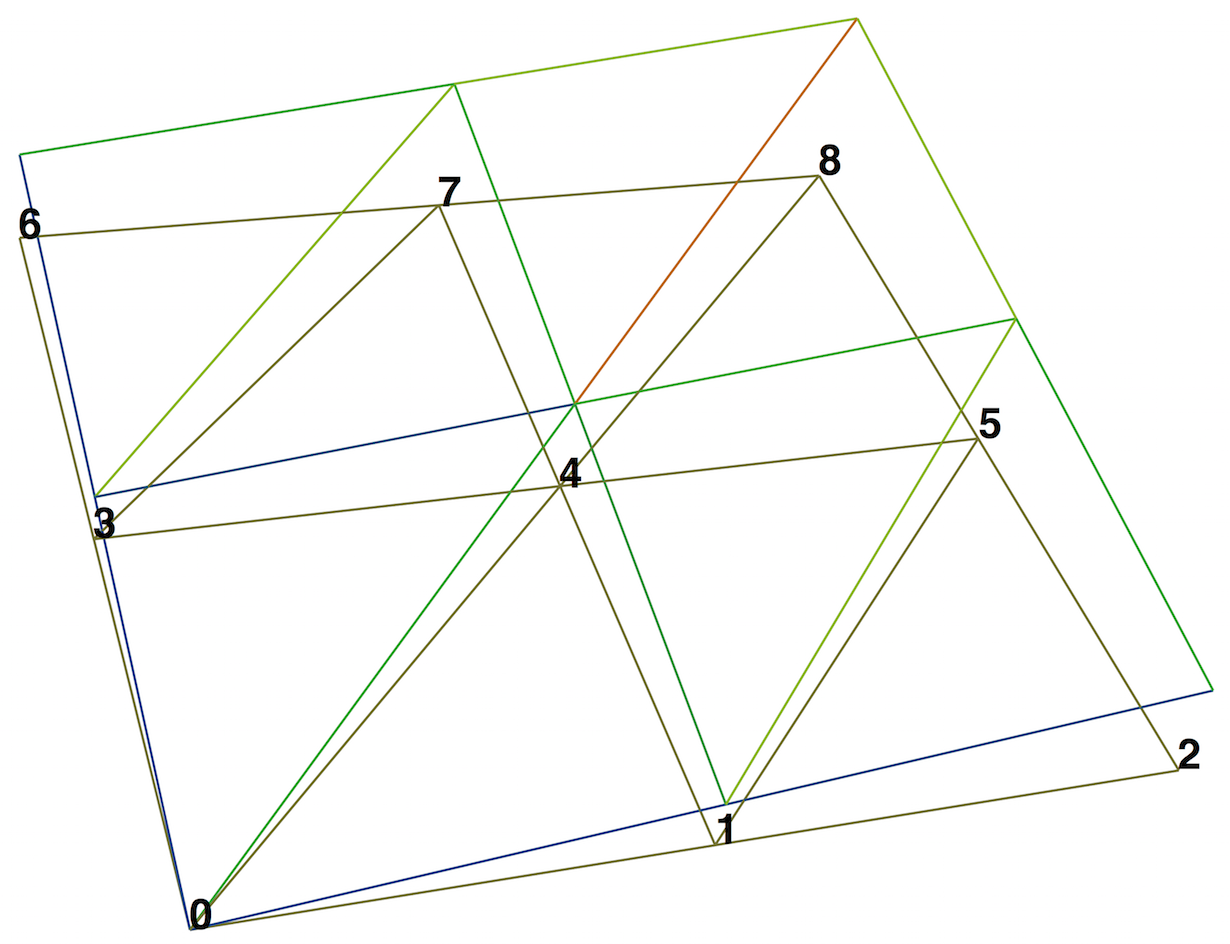
\includegraphics[width=0.75\linewidth]{fig/vertex_numbering.png}}

\vspace{6mm}

\index{vertex values}

我们通过调用来检查值
\verb!u.compute_vertex_values!:

\begin{python}
>>> vertex_values = u.compute_vertex_values()
>>> for i, x in enumerate(coordinates):
...     print('vertex %d: vertex_values[%d] = %g\tu(%s) = %g' %
...           (i, i, vertex_values[i], x, u(x)))
vertex 0: vertex_values[0] = 0          u([ 0.  0.]) = 8.46545e-16
vertex 1: vertex_values[1] = 0.5        u([ 0.5  0. ]) = 0.5
vertex 2: vertex_values[2] = 1          u([ 1.  0.]) = 1
vertex 3: vertex_values[3] = 0.5        u([ 0.   0.5]) = 0.5
vertex 4: vertex_values[4] = 1          u([ 0.5  0.5]) = 1
vertex 5: vertex_values[5] = 1.5        u([ 1.   0.5]) = 1.5
vertex 6: vertex_values[6] = 1          u([ 0.  1.]) = 1
vertex 7: vertex_values[7] = 1.5        u([ 0.5  1. ]) = 1.5
vertex 8: vertex_values[8] = 2          u([ 1.  1.]) = 2
\end{python}

\index{vertex to dof map}
\index{dof to vertex map}

我们可以要求FEniCS给我们从顶点到度数的映射
某个功能空间的自由$V$:

\begin{python}
v2d = vertex_to_dof_map(V)
\end{python}
现在,\verb!nodal_values[v2d[i]]! 会给我们带来的价值
自由
对应于顶点\texttt{i}(\texttt{v2d[i]})。 特别是\verb!nodal_values[v2d]!
是具有相同(顶点编号)顺序的所有元素的数组
作为\texttt{coordinates}。 逆映射,从自由度数到
顶点数由\verb!dof_to_vertex_map(V)!给出。 这意味着
我们可以打电话\verb!coordinates[dof_to_vertex_map(V)]! 得到所有的数组
坐标与自由度相同。 注意
这些映射仅适用于$\mathsf{P}_1$元素的FEniCS。

对于Lagrange度数大于1的元素,有度数
自由度(节点)不对应于顶点。 对于这些
元素,我们可以通过调用获得顶点值
\verb!u.compute_vertex_values(mesh)!,我们可以获得自由度
通过调用\texttt{u.vector()。array()}。 获取坐标相关联
我们需要对所有的自由度进行迭代
网格并要求FEniCS返回与之相关的坐标和自由度
与每个元素(单元格)。 此信息存储在
\texttt{FunctionSpace}的\texttt{FiniteElement}和\texttt{DofMap}对象。该
以下代码说明了如何迭代网格的所有元素
并打印与之相关的坐标和自由度
元件。

\begin{python}
element = V.element()
dofmap = V.dofmap()
for cell in cells(mesh):
    print(element.tabulate_dof_coordinates(cell))
    print(dofmap.cell_dofs(cell.index()))
\end{python}

\subsection{设定自由度}

我们已经看到了如何在\texttt{numpy}数组中提取节点值。
如果需要,我们也可以调整节点值。 说我们想要
规范化解决方案,使$\max_j |U_j| = 1$。 然后我们
必须划分所有$U_j$值
由$\max_j |U_j|$。 以下功能执行任务:

\begin{python}
def normalize_solution(u):
    "Normalize u: return u divided by max(u)"
    u_array = u.vector().array()
    u_max = np.max(np.abs(u_array))
    u_array /= u_max
    u.vector()[:] = u_array
    #u.vector().set_local(u_array)  # alternative
    return u
\end{python}
当使用Lagrange元素时,这个(大约)确保了
函数$u$的最大值为$1$。

\texttt{/ =}运算符意味着
在左边的对象的就地修改:全部
数组元素\verb!nodal_values! 按值\verb!u_max!划分。
或者,我们可以做\verb!nodal_values = nodal_values / u_max!,其中
意味着在右边创建一个新的数组并分配这个
数组命名为\verb!nodal_values!。

\begin{notice}[操纵自由度时要小心]
一个像\texttt{u.vector()。array()}的调用返回一个数据的副本
\texttt{u.vector()}。 因此,必须永远不要执行任务
\texttt{u.vector.array()[:] = ...},而是提取\texttt{numpy}数组
(即复制),操作它,并用\texttt{u.vector()[:] = }插入,
或使用\verb!u.set_local(...)!。
\end{notice}

\subsection{功能评估}

\index{function evaluation}

FEniCS \texttt{Function}对象在内部是唯一定义的
的有限元网格的每个单元格。 对于连续(Lagrange)
函数空间,函数值也是唯一定义的
细胞界限 可以简单地对\texttt{Function}对象\texttt{u}进行评估
调用

\begin{python}
u(x)
\end{python}
\texttt{x}是\texttt{Point}或正确空间的Python元组
尺寸。 当\texttt{Function}被评估时,FEniCS必须首先查找
包含给定点(如果有)的网格的单元格,以及
然后评估给定的基函数的线性组合
指向有问题的单元格内。 FEniCS使用高效数据
结构(边界框树)快速找到点,但是
建造树是一个相对昂贵的操作,所以成本
在单点评估\texttt{Function}是很昂贵的。 重复
评估将重用计算的数据结构,从而
相对较便宜。

\begin{notice}[廉价vs昂贵的功能评估]
一个\texttt{Function}对象
\texttt{u}可以以各种方式进行评估:

\begin{enumerate}
\item \texttt{u(x)}为任意点\texttt{x}

\item \texttt{u.vector().array()[i]}自由度数\texttt{i}

\item \verb!u.compute_vertex_values()[i]! 在顶点编号\texttt{i}
\end{enumerate}

\noindent
第一种方法虽然非常灵活,但通常是昂贵的
而另外两个是非常有效的(但限于某些点)。
\end{notice} 

为了演示使用\texttt{Function}对象的点评估,我们
打印计算有限元解的值\texttt{u}
Poisson问题在域的中心点,并与之进行比较
确切的解决方案:

\begin{python}
center = (0.5, 0.5)
error = u_D(center) - u(center)
print('Error at %s: %g' % (center, error))
\end{python}
一个$2\times(3\times 3)$
网格,输出
以前的片段变成了

\begin{python}
Error at (0.5, 0.5): -0.0833333
\end{python}
差异是由于中心点不是节点
在这个特定的网格中,而是细胞内部的一个点
\texttt{u}在\verb!u_D!的细胞上线性变化! 是一个二次方
功能。 当中心点是一个节点时,如$2\times(2\times
2)$或$2\times(4\times 4)$
网格,错误是顺序的
$10 ^{ - 15}$。

\section{后处理计算}
\label{ftut:possion:2D:varcoeff}

\index{postprocessing}
\index{ft10\_poisson\_extended.py@{\rm\texttt{ft10\_poisson\_extended.py}}}

作为本章的最后一个主题,我们将看看如何
后处理计算; 那就是如何计算各种派生的
来自PDE的计算溶液的量。 解决方案$u$
本身可能是可视化的一般特征的兴趣
解决方案,但有时一个人对计算解决方案感兴趣
用于计算从解决方案中导出的特定数量的PDE,
例如,通量,点值或某些平均值
解。

\subsection{测试问题}

作为测试问题,我们再次考虑可变系数Poisson
单个Dirichlet边界条件的问题:

\begin{alignat}{2}
    - \nabla\cdot(\kappa\nabla u) &= f \quad &&\mbox{in } \Omega,
\label{ch:poisson0:2D:varcoeff} \\
    u &= \ub \quad &&\mbox{on}\  \partial\Omega\tp
\end{alignat}
让我们继续使用我们最喜欢的解决方案$u(x,y)=1+x^2+2y^2$和
然后开出$\kappa(x,y)=x+y$。 它遵循
$\ub(x,y)=1+x^2+2y^2$和$f(x,y)=-8x-10y$。

像以前一样,这个模型问题的变分公式
可以在FEniCS中指定为

\begin{python}
a = kappa*dot(grad(u), grad(v))*dx
L = f*v*dx
\end{python}
系数为$\kappa$,右边为$f$

\begin{python}
kappa = Expression('x[0] + x[1]', degree=1)
f = Expression('-8*x[0] - 10*x[1]', degree=1)
\end{python}

\subsection{通量计算}
\label{ch:poisson0:gradu}

计算通量$Q=-\kappa\nabla u$通常是有意义的。
由于$u=\sum_{j=1}^N U_j \phi_j$,因此

\begin{equation*}
Q = -\kappa\sum_{j=1}^N U_j \nabla \phi_j\tp
\end{equation*}
我们注意到分段连续有限元标量的梯度
因为基函数是一个不连续的矢量场
$\{\phi_j\}$在边界处有不连续的派生词
细胞。 例如,使用1级的Lagrange元素,$u$是线性的
在每个细胞上,梯度变成分段
恒定矢量场。 相反,确切的梯度是
连续。 为了可视化和数据分析的目的,我们经常
希望计算的梯度是一个连续的矢量场。通常情况下,
我们想要$\nabla u$的每个组件
以相同的方式表示
作为$u$本身。 为此,我们可以投影组件
$\nabla u$与我们用于$u$的功能空间相同。 这意味着
我们解决$w=\nabla u$
大约通过有限元法,
对于$w$的组件使用相同的元素,就像我们所使用的那样
$u$。 这个过程称为\emph{projection}。

\index{project@{\rm\texttt{project}}}

Projection是有限元分析中的常用操作,
我们已经看过,FEniCS
具有轻松执行projection的功能:
\texttt{project(expression, W)},它返回一些projection
表达进空格\texttt{W}。

在我们的情况下,通量$Q=-\kappa\nabla u$
是向量值的,我们需要选择\texttt{W}作为向量值函数
与\texttt{u}所在的空格\texttt{V}相同程度的空间:

\begin{python}
V = u.function_space()
mesh = V.mesh()
degree = V.ufl_element().degree()
W = VectorFunctionSpace(mesh, 'P', degree)

grad_u = project(grad(u), W)
flux_u = project(-k*grad(u), W)
\end{python}

投影的应用很多,包括不连续的转动
梯度场变为连续的,比较高阶和低阶
函数近似,并转换高阶有限元
解决了一个分段线性场,这是许多需要的
可视化包。

绘制通量矢量场自然就像绘图一样简单
还要别的吗:

\begin{python}
plot(flux_u, title='flux field')

flux_x, flux_y = flux_u.split(deepcopy=True)  # extract components
plot(flux_x, title='x-component of flux (-kappa*grad(u))')
plot(flux_y, title='y-component of flux (-kappa*grad(u))')
\end{python}
\texttt{deepcopy=True}参数表示\emph{deep copy},它是
计算机科学的一般术语意味着数据的副本是
回。 (相反的,\texttt{deepcopy=False},
意思是\emph{shallow copy},其中
返回的对象只是指向原始数据的指针。)

\index{degrees of freedom}
\index{nodal values}

对于通量场的节点值的数据分析,我们可以
抓取底层的\texttt{numpy}数组(需要一个\texttt{deepcopy=True}
在\texttt{flux}的分割中):

\begin{python}
flux_x_nodal_values = flux_x.vector().dofs()
flux_y_nodal_values = flux_y.vector().dofs()
\end{python}
自由度\verb!flux_u! 矢量场也可以
达到了

\begin{python}
flux_u_nodal_values = flux_u.vector().array()
\end{python}
但是,这是一个包含度数的\texttt{numpy}数组
自由的$x$和$y$组件的通量和
FEniCS可以将组件的顺序混合起来
提高计算效率。

功能\verb!demo_flux! 在程序中
\begin{center}
\url{https://fenicsproject.org/pub/tutorial/python/vol1/ft10_poisson_extended.py}
\end{center}
演示了上述计算。

\begin{notice}[手动投影。]
虽然您将始终使用\texttt{project}来投影有限元素
功能,看看如何制定它可以是有启发性的
在数学上投影并在FEniCS中手动执行其步骤。

假设我们有一个表达式$g = g(u)$,我们想要项目
进入一些空间$W$。 ($L^2$)的数学公式
投影$w = P_W g$成$W$是变分问题

\begin{equation}
  \int_{\Omega} w v \dx = \int_{\Omega} g v \dx
\end{equation}
对于所有测试函数$v\in W$。 换句话说,我们有一个
标准变量问题$a(w, v) = L(v)$现在

\begin{align}
a(w, v) &= \int_\Omega w v \dx,\\
L(v) &= \int_\Omega g v \dx\tp
\end{align}
注意,当$W$中的函数是向量值的时候,就像这样
当我们投影渐变$g(u) = \nabla u$时,我们必须替换
以上产品由$w\cdot v$和$g\cdot v$。

变异问题在FEniCS中很容易定义。
\begin{python}
w = TrialFunction(W)
v = TestFunction(W)

a = w*v*dx  # or dot(w, v)*dx when w is vector-valued
L = g*v*dx  # or dot(g, v)*dx when g is vector-valued
w = Function(W)
solve(a == L, w)
\end{python}
\texttt{solve}的边界条件参数被丢弃
这个问题没有必要的边界条件。
\end{notice}

\subsection{计算功能}
\label{ch:poisson0:functionals}
\index{functionals}

在计算了PDE的解决方案$u$之后,我们偶尔想要计算
$u$的功能,例如,

\begin{equation}
{1\over2}||\nabla u||^2 = {1\over2}\int_\Omega \nabla u\cdot \nabla u \dx,
\label{ch:poisson0:functionals:energy}
\end{equation}
这通常反映了一些能量。
另一个经常出现的功能是错误

\begin{equation}
||\uex-u|| = \left(\int_\Omega (\uex-u)^2 \dx\right)^{1/2},
\label{ch:poisson0:functionals:error}
\end{equation}
其中$\uex$是确切的解决方案。 这个错误是特别的
研究有限元收敛性时的兴趣
方法。 其他时候,我们可能会对计算感兴趣
通过一部分流出
$\Gamma$的边界$\partial\Omega$,

\begin{equation}
F = -\int_\Gamma \kappa\nabla u\cdot n \ds,
\label{ch:poisson0:functionals:flux}
\end{equation}
其中$n$是$\Gamma$上的向外指向单元。

所有这些功能都很容易用FEniCS进行计算,我们将看到
在下面的例子中。

\index{energy functional}

\paragraph{能量功能。}
能量函数的被积函数
(\ref{ch:poisson0:functionals:energy})在UFL中描述
语言与我们描述的形式相同:

\begin{python}
energy = 0.5*dot(grad(u), grad(u))*dx
E = assemble(energy)
\end{python}
通过调用\texttt{assemble}来评估函数\texttt{energy}
我们以前用来组装矩阵的函数
向量。 FEniCS将会认识到该表单具有“0级”(因为它)
不包含试用和测试功能),并返回结果
标量值。

\index{error functional}

\paragraph{错误功能。}
功能(\ref{ch:poisson0:functionals:error})可以
计算如下:

\begin{python}
error = (u_e - u)**2*dx
E = sqrt(abs(assemble(error)))
\end{python}
确切的解决方案$\uex$在这里由\texttt{Function}或
\texttt{Expression}对象
\verb!u_e!,而\texttt{u}是有限元
近似(因此也是一个\texttt{Function})。 有时,非常小
错误值,\texttt{assemble(error)}的结果可以是(非常小的)
负数,所以我们在\texttt{E}的表达式中使用了\texttt{abs}
以确保\texttt{sqrt}函数的正值。

\index{errornorm@{\rm\texttt{errornorm}}}

正如在~\ref{ch:poisson0:convrates}部分中所解释和演示的,\verb!(u_e - u)**2*dx!可能导致太乐观的收敛速度,除非有一个小心点
差异\verb!u_e - u! 被评估。 一般建议
为了可靠的错误计算是使用\texttt{errornorm}函数:

\begin{python}
E = errornorm(u_e, u)
\end{python}

\index{flux functional}

\paragraph{助焊剂功能。}
计算通量积分,如$F = -\int_\Gamma \kappa\nabla
u\cdot n \ds$,我们需要定义$n$
向量,在FEniCS中称为\emph{facet normal}。 如果是表面域
$\Gamma$中的通量积分是完整的边界,我们可以执行
通量计算

\begin{python}
n = FacetNormal(mesh)
flux = -k*dot(grad(u), n)*ds
total_flux = assemble(flux)
\end{python}
虽然\texttt{grad(u)}和\verb!nabla_grad(u)! 在上述可互换
当\texttt{u}是一个标量函数时,我们选择写入
\texttt{grad(u)},因为如果我们概括一下,这是正确的表达式
向量PDE的基本方程。 用\verb!nabla_grad(u)! 我们
在这种情况下必须写\verb!dot(n,nabla_grad(u))!

可以将整合限制到边界的一部分
通过使用网格函数来标记相关部分,如下所述
第~\ref{ch:poisson0:multi:bc}。 假设该部分对应
到子域号\texttt{i},变体的相关语法
通量的公式为\texttt{-k*dot(grad(u), n)*ds(i)}。


\begin{notice}[关于整合准确性的说明]
如前所述,FEniCS \texttt{Expressions}必须使用定义
一个特殊的程度 该学位告诉FEniCS到哪个地方
有限元空间的表达式应该是内插的
执行本地计算(集成)。 作为说明,
考虑积分的计算$\int_0^1 \cos x \dx = \sin
1$。 这可以在FEniCS中计算
\begin{python}
mesh = UnitIntervalMesh(1)
I = assemble(Expression('cos(x[0])', degree=degree)*dx(domain=mesh))
\end{python}
请注意,我们必须在这里指定参数\texttt{domain = mesh}
测量\texttt{dx}。 在定义表单时通常不是必需的
在FEniCS中,但是由于\texttt{cos(x[0])}未关联,所以必需
与任何域(如我们集成\texttt{Function}
来自某些\texttt{Mesh}上定义的\texttt{FunctionSpace})。

0和5之间的变化值,$|\sin(1) - I|$的值
\texttt{0.036},
\texttt{0.071},
\texttt{0.00030},
\texttt{0.00013},
\texttt{4.5E-07}, and
\texttt{2.5E-07}.

FEniCS还允许表达式直接表达为一部分
表单。 这需要创建一个\texttt{SpatialCoordinate}。
在这种情况下,精度由准确度决定
集成,可以由\texttt{degree}参数控制
整合度量\texttt{dx}。 \texttt{degree}参数指定
对于该程度的多项式,积分应该是精确的。

以下代码片段显示
如何使用这种方法计算积分$\int_0^1 \cos x \dx$:
\begin{python}
mesh = UnitIntervalMesh(1)
x = SpatialCoordinate(mesh)
I = assemble(cos(x[0])*dx(degree=degree))
\end{python}
0和5之间的变化值,$|\sin(1) - I|$的值
\texttt{0.036},
\texttt{0.036},
\texttt{0.00020},
\texttt{0.00020},
\texttt{4.3E-07},
\texttt{4.3E-07}.
请注意,正交程度仅适用于
奇数,以便$0$的程度将使用相同的正交
规则为$1$,
学位$2$将给出相同的正交规则为度$3$等等。
\end{notice}

\subsection{计算收敛速度}
\label{ch:poisson0:convrates}

\index{convergence rate}

任何数值方法的核心问题是它的\emph{convergence rate}:
当分辨率为零时,误差逼近为零
增加? 对于有限元方法,这通常对应于
从理论上或经验证明,错误$e = \uex - u$
被网格大小$h$限制到某些权力$r$; 也就是$\|e\|
\leq C h^r$为一些常数$C$。 数字$r$被称为
\emph{convergence rate}的方法。 注意不同的规范,像
$L^2$-规范$\|e\|$或$H^1_0$-标准$\|\nabla e\|$通常有
收敛速度不同。

为了说明如何在FEniCS中计算误差和收敛速度,
我们已经包含了函数\verb!compute_convergence_rates! 在里面
教程课程
\begin{center}
\url{https://fenicsproject.org/pub/tutorial/python/vol1/ft10_poisson_extended.py}。
\end{center}
这是一种在验证有限元代码时非常方便的工具
因此将在此详细解释。

\paragraph{计算错误规范。}
\index{error}
\index{norm}

正如我们已经看到的,$L^2$-错误的规范$\uex - u$
能够在FEniCS中实施

\begin{python}
error = (u_e - u)**2*dx
E = sqrt(abs(assemble(error)))
\end{python}
如上所述,我们在\texttt{E}的表达式中使用了\texttt{abs}来确保
\texttt{sqrt}函数的正值。

了解FEniCS计算错误是非常重要的
上面的代码,因为我们可能会在使用时遇到微妙的问题
计算收敛速度的价值。 第一个微妙的问题是
如果\verb!u_e! 不是一个有限元素的函数(一个创建的对象)
使用\texttt{Function(V)}),如果\verb!u_e! 被定义为
\texttt{Expression},FEniCS必须插入\verb!u_e! 变成一些局部有限的
网格的每个元素上的元素空间。 用于的程度
插值是由强制关键字参数决定的
\texttt{Expression}类,例如:

\begin{python}
u_e = Expression('sin(x[0])', degree=1)
\end{python}
这意味着计算出的误差将不等于实际值
错误$\|\uex - u\|$而是有限的差异
元素解决方案$u$和分段线性插值
$\uex$。 这可能会产生太乐观(太小)的价值
错误。 通过内插精确度可以获得更好的价值
解决方案进入高阶函数空间,这可以通过
简单地增加学位:

\begin{python}
u_e = Expression('sin(x[0])', degree=3)
\end{python}

第二个微妙的问题是当FEniCS评估表达式时
\verb!(u_e - u)** 2!,这将被扩展为\\\verb!u_e**2 + u**2 - 2*u_e*u! 如果错误很小(解决方案本身就是
中等大小),这个计算将对应于减法
两个正数(\verb!u_e**2 + u**2! $\sim 1$ and \verb!2*u_e*u! $\sim
1$)产生少量。 这样的计算很容易
四舍五入的错误,这可能再次导致不可靠的价值
错误。 为了使这种情况更糟,FEniCS可能会扩大这一点
计算大量的术语,特别是较高的
订单元素,使计算非常不稳定。

为了帮助解决这些问题,FEniCS提供了内置的功能
\texttt{errornorm},它以更智能的方式计算错误规范
办法。 首先,两个\verb!u_e! 和\texttt{u}被插入到高阶
功能空间。 然后,\verb!u_e!的自由度 和\texttt{u}是
减去在高阶函数中产生新的函数
空间。 最后,FEniCS整合了平方的差异
函数,然后取平方根来获取错误的值
规范。 使用\texttt{errornorm}功能很简单:

\begin{python}
E = errornorm(u_e, u, normtype='L2')
\end{python}
这是一个简短的实现\texttt{errornorm}的说明:

\begin{python}
def errornorm(u_e, u):
    V = u.function_space()
    mesh = V.mesh()
    degree = V.ufl_element().degree()
    W = FunctionSpace(mesh, 'P', degree + 3)
    u_e_W = interpolate(u_e, W)
    u_W = interpolate(u, W)
    e_W = Function(W)
    e_W.vector()[:] = u_e_W.vector().array() - u_W.vector().array()
    error = e_W**2*dx
    return sqrt(abs(assemble(error)))
\end{python}

有时候计算错误是有意义的
渐变字段:$||\nabla(\uex-u)||$,
通常被称为$H^1_0$或$H^1$
错误的seminorm。
这可以用上面的表达式来代替
\texttt{error} 通过\verb!error = dot(grad(e_W), grad(e_W))*dx!,或通过调用
在FEniCS中的\texttt{errornorm}:

\begin{python}
E = errornorm(u_e, u, norm_type='H10')
\end{python}
有关可用的更多信息,请在Python中键入\texttt{help(errornorm)}
规范类型。

函数\verb!compute_errors! 在
\begin{center}
\url{https://fenicsproject.org/pub/tutorial/python/vol1/ft10_poisson_extended.py}
\end{center}
说明了FEniCS中各种误差规范的计算。

\paragraph{计算收敛速度。}
我们来研究如何在FEniCS中计算收敛速度。
\texttt{solver}函数
\begin{center}
\url{https://fenicsproject.org/pub/tutorial/python/vol1/ft10_poisson_extended.py}
\end{center}
使我们能够轻松地为更精细和更细的网格计算解决方案
使我们能够研究收敛速度。 定义元素大小
$h=1/n$,其中$n$是$x$和$y$中的单元格分隔数
方向(\texttt{n = Nx = Ny})。 我们进行实验
$h_0>h_1>h_2>\cdots$并计算相应的错误$E_0, E_1,
E_2$等等。 假设$E_i=Ch_i^r$为未知常数$C$和
$r$,我们可以比较两个连续的实验,$E_{i-1}=Ch_{i-1}^r$
和$E_i=Ch_i^r$,并解决$r$:

\begin{equation*}
r = {\ln(E_i/E_{i-1})\over\ln (h_i/h_{i-1})}\tp
\end{equation*}
$r$值应接近预期收敛速度
(通常为$L^2$的多项式度+1)
错误)为$i$
增加。

以上过程可以很容易地转化为Python代码。 这里
我们通过元素度量列表($\mathsf{P}_1$,
$\mathsf{P}_2$和$\mathsf{P}_3$),
对一系列细化的网格进行实验
每个实验报告由\verb!compute_errors!返回的六个错误类型。

\paragraph{测试问题。}
为了说明收敛速度的计算,我们选择一个
精确的解决方案$\uex$,这个时间比一点更有趣
对于~\ref{ch:fundamentals}中的测试问题:

\begin{equation*}
\uex(x,y) = \sin(\omega\pi x)\sin(\omega\pi y).
\end{equation*}
这个选择意味着$f(x,y)=2\omega^2\pi^2 u(x,y)$。
将$\omega$限制为整数,
因此边界值由$\ub=0$给出。

我们需要定义适当的边界条件,确切的
解决方案和代码中的$f$函数:

\begin{python}
def boundary(x, on_boundary):
    return on_boundary

bc = DirichletBC(V, Constant(0), boundary)

omega = 1.0
u_e = Expression('sin(omega*pi*x[0])*sin(omega*pi*x[1])',
                 degree=6, omega=omega)

f = 2*pi**2*omega**2*u_e
\end{python}

\paragraph{实验。}
可以实现收敛速度的计算
在函数\verb!demo_convergence_rates!中找到 在演示程序中
\begin{center}
\url{https://fenicsproject.org/pub/tutorial/python/vol1/ft10_poisson_extended.py}。
\end{center}
我们取得一些有趣的结果。
使用无限度的自由度差异规范,
我们获得下表:

{\small

\vspace{4mm}

\begin{tabular}{lrrrr}
\hline\noalign{\smallskip}
\multicolumn{1}{c}{ element } & \multicolumn{1}{c}{ $n=8\ $ } & \multicolumn{1}{c}{ $n=16\ $ } & \multicolumn{1}{c}{ $n=32\ $ } & \multicolumn{1}{c}{ $n=64\ $ } \\
\noalign{\smallskip}\hline\noalign{\smallskip}
$\mathsf{P}_1$ & 1.99    & 2.00     & 2.00     & 2.00     \\
$\mathsf{P}_2$ & 3.99    & 4.00     & 4.00     & 4.01     \\
$\mathsf{P}_3$ & 3.95    & 3.99     & 3.99     & 3.92     \\
\noalign{\smallskip}\hline\noalign{\smallskip}
\end{tabular}

\vspace{4mm}

}

\noindent
$n=32$和$\mathsf{P}_3$的条目如3.99表示我们
通过比较两个网格,分辨率来估计3.99的比率
$n=32$和$n=16$,使用$\mathsf{P}_3$元素。 注意
节点上$\mathsf{P}_2$的超会聚。 最好的估计
的价格出现在最右边的列,因为这些费率是
基于最好的决议,因此最深入
渐近的制度(直到我们达到了四舍五入的错误和
线性系统的不精确解决方案开始起作用)。

$L^2$-使用FEniCS计算的范数误差
\texttt{errornorm}功能显示
$u$的预期$h^{d+1}$率:

{\small

\vspace{4mm}

\begin{tabular}{lrrrr}
\hline\noalign{\smallskip}
\multicolumn{1}{c}{ element } & \multicolumn{1}{c}{ $n=8\ $ } & \multicolumn{1}{c}{ $n=16\ $ } & \multicolumn{1}{c}{ $n=32\ $ } & \multicolumn{1}{c}{ $n=64\ $ } \\
\noalign{\smallskip}\hline\noalign{\smallskip}
$\mathsf{P}_1$ & 1.97    & 1.99     & 2.00     & 2.00     \\
$\mathsf{P}_2$ & 3.00    & 3.00     & 3.00     & 3.00     \\
$\mathsf{P}_3$ & 4.04    & 4.02     & 4.01     & 4.00     \\
\noalign{\smallskip}\hline\noalign{\smallskip}
\end{tabular}

\vspace{4mm}

}

\noindent
但是,使用\verb!(u_e - u)**2! 对于误差计算,用相同的
\verb!u_e!插值的程度 对于\texttt{u},给出奇怪的
结果:

{\small   % for Springer style: small table font and more vspace

\vspace{4mm}

\begin{tabular}{lrrrr}
\hline\noalign{\smallskip}
\multicolumn{1}{c}{ element } & \multicolumn{1}{c}{ $n=8\ $ } & \multicolumn{1}{c}{ $n=16\ $ } & \multicolumn{1}{c}{ $n=32\ $ } & \multicolumn{1}{c}{ $n=64\ $ } \\
\noalign{\smallskip}\hline\noalign{\smallskip}
$\mathsf{P}_1$ & 1.97    & 1.99     & 2.00     & 2.00     \\
$\mathsf{P}_2$ & 3.00    & 3.00     & 3.00     & 3.01     \\
$\mathsf{P}_3$ & 4.04    & 4.07     & 1.91     & 0.00     \\
\noalign{\smallskip}\hline\noalign{\smallskip}
\end{tabular}

\vspace{4mm}

}

\noindent
这是一个例子,重要的是插入\verb!u_e! 到一个
高阶空间(3阶多项式在这里就足够了)。 这个
通过使用\texttt{errornorm}函数自动处理。

检查收敛速度是验证PDE的极好方法
码。

\subsection{利用结构化网格数据}
\label{ftut:structviz}
\index{structured mesh}
\index{visualization, structured mesh}
\index{scitools@{\rm\texttt{scitools}}}

许多读者在可视化和数据方面有丰富的经验
分析1D,2D和3D标量和矢量场均匀,
结构化网格,而FEniCS解决方案专门工作
非结构化网格 由于它可以很多次实践
使用结构化数据,我们在本节中讨论如何
提取用于计算的有限元解的结构化数据
FENICS。

\index{BoxField@{\rm\texttt{BoxField}}}

必要的第一步是将我们的\texttt{Mesh}对象转换为对象
表示具有同样形状的矩形(或3D框)
矩形细胞。 第二步是转变
节点值的一维数组为二维数组
将值保存在结构化的单元格的角落
目。 我们要通过$i$和$j$索引$i$来访问一个值
计数$x$方向的单元格,$j$计数$y$中的单元格
方向。 但这种转变原则上是直截了当的
它经常导致模糊的索引错误,所以使用软件
减轻工作的工具是有利的。

在本书附带的示例程序目录中,我们有
包括Python模块
\begin{center}
\url{https://fenicsproject.org/pub/tutorial/python/vol1/boxfield.py}
\end{center}
它提供了用于处理结构化网格数据的实用程序
FENICS。 给定有限元函数\texttt{u},以下函数
在结构化网格上返回表示\texttt{u}的\texttt{BoxField}对象:

\begin{python}
from boxfield import *
u_box = FEniCSBoxField(u, (nx, ny))
\end{python}

\verb!u_box! 对象包含几个有用的数据结构:

\begin{itemize}
 \item \verb!u_box.grid!: 对象为结构化网格

 \item \verb!u_box.grid.coor[X]!: \texttt{X=0}方向的网格坐标

 \item \verb!u_box.grid.coor[Y]!: \texttt{Y=1}方向的网格坐标

 \item \verb!u_box.grid.coor[Z]!: \texttt{Z=2}方向的网格坐标

 \item \verb!u_box.grid.coorv[X]!: \verb!u_box.grid.coor[X]!的矢量化版本

 \item \verb!u_box.grid.coorv[Y]!: \verb!u_box.grid.coor[Y]!的矢量化版本

 \item \verb!u_box.grid.coorv[Z]!: \verb!u_box.grid.coor[Z]!的矢量化版本

 \item \verb!u_box.values!: \texttt{numpy}数组,保存\texttt{u}值;
   \verb!u_box.values[I,J]! 在网格点保持\texttt{u},坐标为\\
    \verb!(u_box.grid.coor[X][i], u_box.grid.coor[Y][j])!
\end{itemize}

\noindent
\paragraph{迭代点数和值。}
现在让我们使用\texttt{solver}函数
\begin{center}
\url{https://fenicsproject.org/pub/tutorial/python/vol1/ft10_poisson_extended.py}
\end{center}
代码来计算\texttt{u},将其映射到一个\texttt{BoxField}对象上的结构化
网格表示,并打印坐标和函数值
在所有网格点:

\begin{python}
u = solver(p, f, u_b, nx, ny, 1, linear_solver='direct')
u_box = structured_mesh(u, (nx, ny))
u_ = u_box.values

# Iterate over 2D mesh points (i, j)
for j in range(u_.shape[1]):
    for i in range(u_.shape[0]):
        print('u[%d, %d] = u(%g, %g) = %g' %
              (i, j,
               u_box.grid.coor[X][i], u_box.grid.coor[Y][j],
               u_[i, j]))
\end{python}

\paragraph{计算有限差分近似。}
使用多维数组\verb!u_ = u_box.values!, 我们可以轻松地
表示衍生物的有限差分近似:

\begin{python}
x = u_box.grid.coor[X]
dx = x[1] - x[0]
u_xx = (u_[i - 1, j] - 2*u_[i, j] + u_[i + 1, j]) / dx**2
\end{python}

\index{surface plot (structured mesh)}

\paragraph{制作曲面图。}
作为结构化数据访问有限元字段的能力
在许多情况下很方便,例如用于可视化和数据分析。
使用Matplotlib,我们可以创建一个曲面图,如图所示
图~\ref{ftut:structviz:fig1}(左上):

\begin{python}
import matplotlib.pyplot as plt
from mpl_toolkits.mplot3d import Axes3D  # necessary for 3D plotting
from matplotlib import cm
fig = plt.figure()
ax = fig.gca(projection='3d')
cv = u_box.grid.coorv  # vectorized mesh coordinates
ax.plot_surface(cv[X], cv[Y], u_, cmap=cm.coolwarm,
                rstride=1, cstride=1)
plt.title('Surface plot of solution')
\end{python}
关键问题是知道曲面所需的坐标
情节在\verb!u_box.grid.coorv! 并且值在\verb!u_!中。

\begin{figure}[!ht]  % ftut:structviz:fig1
 \centerline{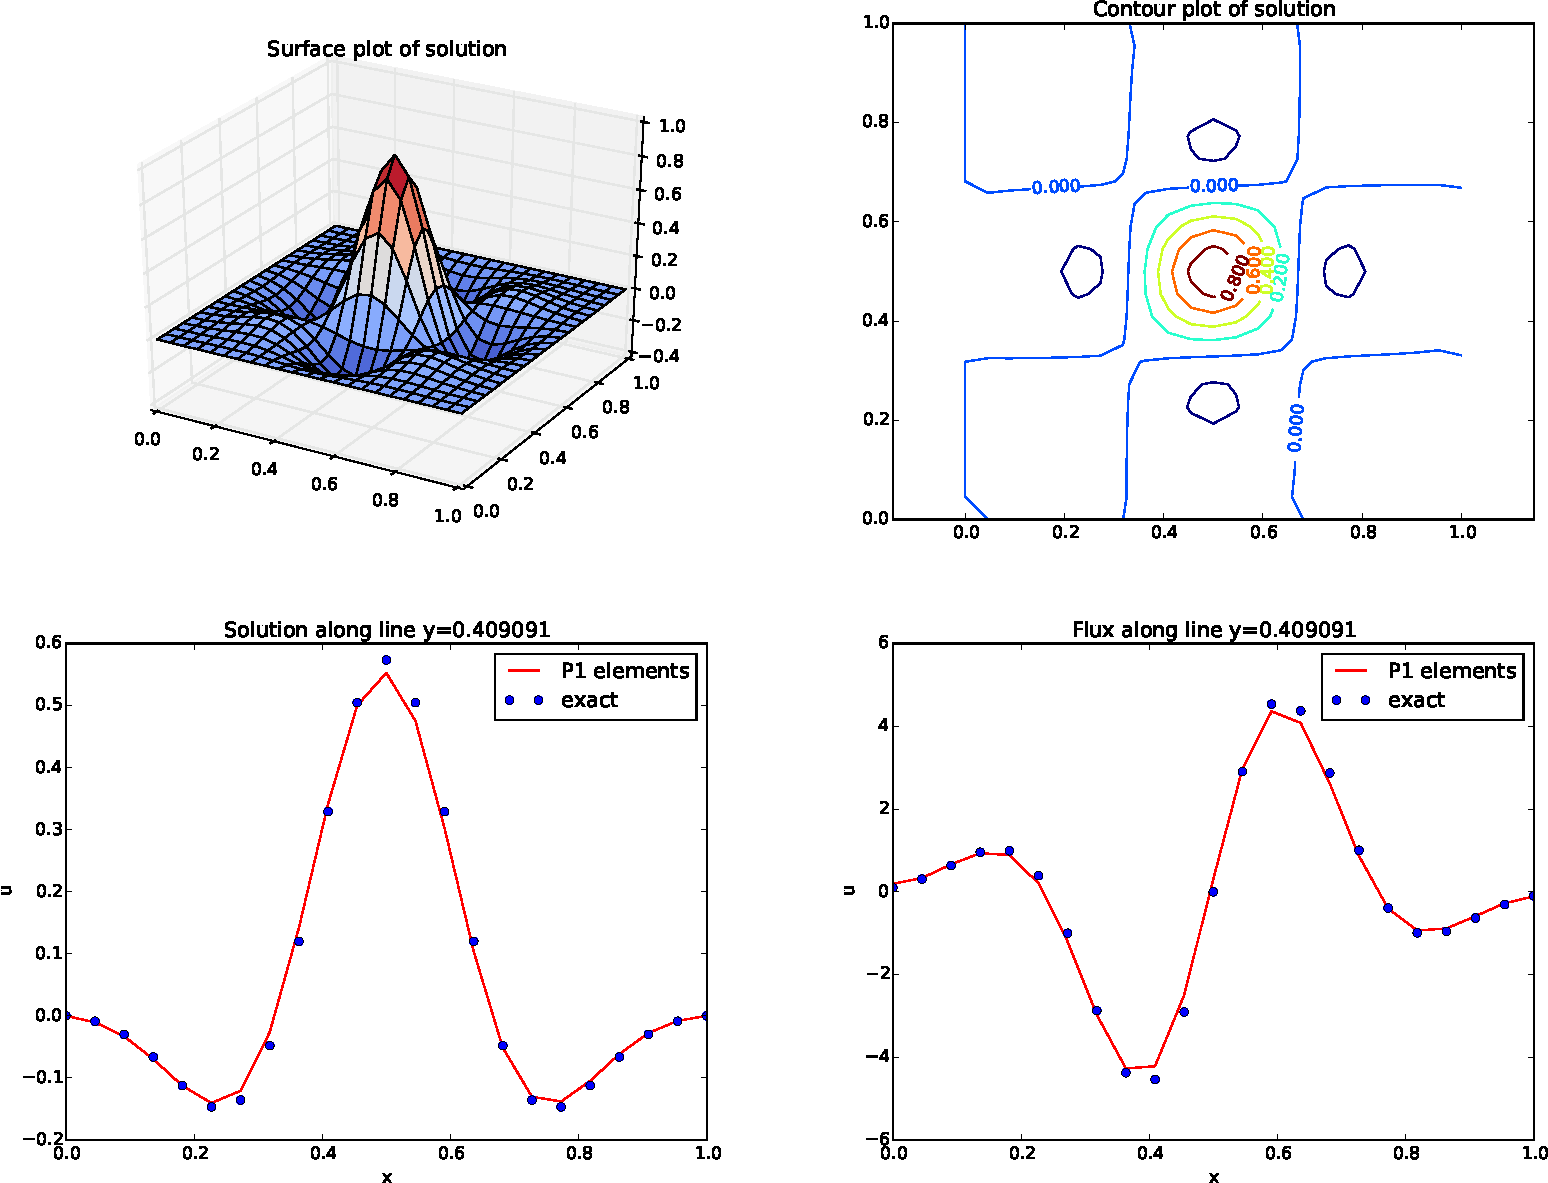
\includegraphics[width=0.95\linewidth]{fig/poisson_extended.pdf}}
 \caption{
 在结构化网格上的各种解决方案。\label{ftut:structviz:fig1}
 }
\end{figure}

\index{contour plot}

\paragraph{制作轮廓图。}
一个轮廓图也可以由Matplotlib制作:

\begin{python}
fig = plt.figure()
ax = fig.gca()
levels = [1.5, 2.0, 2.5, 3.5]
cs = ax.contour(cv[X], cv[Y], u_, levels=levels)
plt.clabel(cs)  # add labels to contour lines
plt.axis('equal')
plt.title('Contour plot of solution')
\end{python}
结果如图~\ref{ftut:structviz:fig1}(右上)所示。

\paragraph{通过域进行曲线图。}
\texttt{BoxField}对象的一个方便的功能是启动的能力
指向域中的方向,然后提取字段和
沿\emph{mesh points}最近行的相应坐标。 我们有
已经看到如何在网格中沿线插入解决方案,但是
使用\texttt{BoxField},您可以选择计算点(顶点)
检查这些要点。 数值方法经常表现出改善的行为
在这样的点,所以这是有趣的。 对于3D字段
还可以在平面中提取数据。

说我们要绘制$u$
行$y=0.4$。 网格点,\texttt{x}和$ u $值
沿着这一行,\verb!u_val!,可以被提取出来


\begin{python}
start = (0, 0.4)
x, u_val, y_fixed, snapped = u_box.gridline(start, direction=X)
\end{python}
如果行被贴到最接近的位置,则变量\texttt{snapped}为true
网格线,在这种情况下\verb!y_fixed! 持有攫取
(改变)$y$值。 关键字参数\texttt{snap}默认情况下为\texttt{True}
以避免插补和力捕捉。

沿线的数值和精确解的比较
$y\approx 0.41$(从$y=0.4$中扣除)由以下代码制成:

\begin{python}
    # Plot u along a line y = const and compare with exact solution
    start = (0, 0.4)
    x, u_val, y_fixed, snapped = u_box.gridline(start, direction=X)
    u_e_val = [u_D((x_, y_fixed)) for x_ in x]
    plt.figure()
    plt.plot(x, u_val, 'r-')
    plt.plot(x, u_e_val, 'bo')
    plt.legend(['P1 elements', 'exact'], loc='best')
    plt.title('Solution along line y=%g' % y_fixed)
    plt.xlabel('x');  plt.ylabel('u')
\end{python}
对于所得曲线图,请参见图~\ref{ftut:structviz:fig1}(左下)。

\paragraph{制作通量的曲线图。}
我们还可以比较数值和
精确通量$-\kappa\partial u/\partial x$与上述相同:

\begin{python}
    # Plot the numerical and exact flux along the same line
    flux_u = flux(u, kappa)
    flux_u_x, flux_u_y = flux_u.split(deepcopy=True)
    flux2_x = flux_u_x if flux_u_x.ufl_element().degree() == 1 \
              else interpolate(flux_x,
                   FunctionSpace(u.function_space().mesh(), 'P', 1))
    flux_u_x_box = FEniCSBoxField(flux_u_x, (nx,ny))
    x, flux_u_val, y_fixed, snapped = \
       flux_u_x_box.gridline(start, direction=X)
    y = y_fixed
    plt.figure()
    plt.plot(x, flux_u_val, 'r-')
    plt.plot(x, flux_u_x_exact(x, y_fixed), 'bo')
    plt.legend(['P1 elements', 'exact'], loc='best')
    plt.title('Flux along line y=%g' % y_fixed)
    plt.xlabel('x');  plt.ylabel('u')
\end{python}

在代码片段开头调用的函数\texttt{flux}是
在示例程序中定义
\begin{center}
\url{https://fenicsproject.org/pub/tutorial/python/vol1/ft10_poisson_extended.py}
\end{center}
并将通量内插到功能空间中。

请注意,Matplotlib是绘图包的选择。 随着
统一的界面在
\begin{center}
\url{https://github.com/hplgit/scitools} {SciTools package}
\footnote{\texttt{https://github.com/hplgit/scitools}}
\end{center}
中可以访问Matplotlib,
Gnuplot,MATLAB,OpenDX,VisIt等绘图引擎通过
相同的API。

\index{sympy@{\rm\texttt{sympy}}}

\paragraph{测试问题。}
图中引用的图形~\ref{ftut:structviz:fig1}对应于
规定解的一个测试问题$\uex = H(x)H(y)$,其中

\[ H(x) = e^{-16(x-\frac{1}{2})^2}\sin(3\pi x)\tp\]
相应的右侧$f$是通过插入确切的获得的
解决方案进入PDE并像以前一样进行区分。
虽然很容易进行
用手分解$f$并对结果表达式进行硬编码
在\texttt{Expression}对象中,更可靠的习惯是使用Python
符号计算引擎,SymPy,执行数学和
自动将公式转换为\texttt{Expression}对象的C ++语法。
简要介绍了
第~\ref{ftut:nonlinear:Newton:auto}。

我们从\texttt{sympy}中定义确切的解决方案开始:

\begin{python}
from sympy import exp, sin, pi  # for use in math formulas
import sympy as sym

H = lambda x: exp(-16*(x-0.5)**2)*sin(3*pi*x)
x, y = sym.symbols('x[0], x[1]')
u = H(x)*H(y)
\end{python}
将\texttt{u}的表达式转换为\texttt{Expression}对象的C或C ++语法
需要两个步骤。 首先我们要求表达式的C代码:

\begin{python}
u_code = sym.printing.ccode(u)
\end{python}
打印\verb!u_code! 给出(这里的输出手动分为两部分
线):

\begin{python}
-exp(-16*pow(x[0] - 0.5, 2) - 16*pow(x[1] - 0.5, 2))*
sin(3*M_PI*x[0])*sin(3*M_PI*x[1])
\end{python}
必要的语法调整正在替换
符号\verb!M_PI! 对于\texttt{pi}(或\verb!DOLFIN_PI!)的C/C++中的$\pi$:

\begin{python}
u_code = u_code.replace('M_PI', 'pi')
u_b = Expression(u_code, degree=1)
\end{python}
此后,我们可以随着计算进展
$f = -\nabla\cdot(\kappa\nabla u)$:

\begin{python}
kappa = 1
f = sym.diff(-kappa*sym.diff(u, x), x) + \
    sym.diff(-kappa*sym.diff(u, y), y)
f = sym.simplify(f)
f_code = sym.printing.ccode(f)
f_code = f_code.replace('M_PI', 'pi')
f = Expression(f_code, degree=1)
\end{python}
我们还需要一个Python函数来确定通量
$-\kappa\partial u/\partial x$:

\begin{python}
flux_u_x_exact = sym.lambdify([x, y], -kappa*sym.diff(u, x),
                              modules='numpy')
\end{python}
在调用之前,还要定义\texttt{kappa = Constant(1)}并设置\texttt{nx}和
\texttt{ny}
\texttt{solver}来计算这个问题的有限元解。

\section{下一步}

如果你来了这么远,你就学会了如何写简单
一系列PDE的脚本式求解器,以及如何构造Python
求解器使用功能和单元测试。 解决更复杂的PDE
并且编写一个更全功能的PDE求解器并不难
第一步通常是写一个解析器进行剥离测试
作为一个简单的Python脚本。 随着脚本的成熟和变得越来越多
复杂,现在是考虑设计的时候,特别是如何
将代码模块化,并将其组织成可重复使用的部分
用于构建灵活可扩展的求解器。

在FEniCS网站上,您将找到更多的文档,
更多示例程序,以及高级解算器和应用程序的链接
写在FEniCS之上。 获得灵感并开发自己的求职者
为您最喜欢的应用程序,发布您的代码并分享您的
知识与FEniCS社区和世界!

PS:\emph{请关注FEniCS教程第2卷!}
